\documentclass[12pt]{article}\usepackage[]{graphicx}\usepackage[]{color}
%% maxwidth is the original width if it is less than linewidth
%% otherwise use linewidth (to make sure the graphics do not exceed the margin)
\makeatletter
\def\maxwidth{ %
  \ifdim\Gin@nat@width>\linewidth
    \linewidth
  \else
    \Gin@nat@width
  \fi
}
\makeatother

\definecolor{fgcolor}{rgb}{0.345, 0.345, 0.345}
\newcommand{\hlnum}[1]{\textcolor[rgb]{0.686,0.059,0.569}{#1}}%
\newcommand{\hlstr}[1]{\textcolor[rgb]{0.192,0.494,0.8}{#1}}%
\newcommand{\hlcom}[1]{\textcolor[rgb]{0.678,0.584,0.686}{\textit{#1}}}%
\newcommand{\hlopt}[1]{\textcolor[rgb]{0,0,0}{#1}}%
\newcommand{\hlstd}[1]{\textcolor[rgb]{0.345,0.345,0.345}{#1}}%
\newcommand{\hlkwa}[1]{\textcolor[rgb]{0.161,0.373,0.58}{\textbf{#1}}}%
\newcommand{\hlkwb}[1]{\textcolor[rgb]{0.69,0.353,0.396}{#1}}%
\newcommand{\hlkwc}[1]{\textcolor[rgb]{0.333,0.667,0.333}{#1}}%
\newcommand{\hlkwd}[1]{\textcolor[rgb]{0.737,0.353,0.396}{\textbf{#1}}}%
\let\hlipl\hlkwb

\usepackage{framed}
\makeatletter
\newenvironment{kframe}{%
 \def\at@end@of@kframe{}%
 \ifinner\ifhmode%
  \def\at@end@of@kframe{\end{minipage}}%
  \begin{minipage}{\columnwidth}%
 \fi\fi%
 \def\FrameCommand##1{\hskip\@totalleftmargin \hskip-\fboxsep
 \colorbox{shadecolor}{##1}\hskip-\fboxsep
     % There is no \\@totalrightmargin, so:
     \hskip-\linewidth \hskip-\@totalleftmargin \hskip\columnwidth}%
 \MakeFramed {\advance\hsize-\width
   \@totalleftmargin\z@ \linewidth\hsize
   \@setminipage}}%
 {\par\unskip\endMakeFramed%
 \at@end@of@kframe}
\makeatother

\definecolor{shadecolor}{rgb}{.97, .97, .97}
\definecolor{messagecolor}{rgb}{0, 0, 0}
\definecolor{warningcolor}{rgb}{1, 0, 1}
\definecolor{errorcolor}{rgb}{1, 0, 0}
\newenvironment{knitrout}{}{} % an empty environment to be redefined in TeX

\usepackage{alltt}
\usepackage[T1]{fontenc}
\usepackage{graphicx}
\usepackage{xcolor}
\IfFileExists{upquote.sty}{\usepackage{upquote}}{}
\begin{document}

\title{Simple Linear Regression}

\author{Morgan Smart}



\section{Abstract}

This paper replicates the analysis from Section 3.1 of Chapter 3. \textit{Linear Regression} in ``An Introduction to Statistical Learning'' by James \textit{et al}. Section 3.1 looks at advertising data and assesses: if there is a relationship between advertising budget and sales, how strong the relationship is if it exists, and if the relationship is linear. In Section 3.1 and in this papaer, these questions are answered by computing a simple linear regression of TV advertising budget (in thousands) on Sales (in thousands) and analyzing the regression results as well as analyzing the fit of the regression line on the scatterplot of TV advertising budget against Sales (in thousands).

\section{Introduction}

A simple linear regression is an approach to predicting a quantitative response $Y$ based on a single predictor variable $X$, where $Y$ and $X$ are vectors and each value in $X$ ($x_i$) has a corresponding value in $Y$ ($y_i$). The model assumes that the relationship between $X$ and $Y$ is linear; thus, in order to compute a simple linear regression that has an accurate interpretation, $X$ and $Y$ \textbf{must} have a linear relationship. The simple linear model can be written as $Y \approx \beta_0 + \beta_1X$, where $\beta_0$ is the intercept and $\beta_1$ is the slope and both are constants, unknowns, and together are the model coefficients. The interpretation of $\beta_0$ is the expected mean value of $Y$ without a predictor variable and the interpretation of $\beta_1$ is the change in $Y$ for a unit increase in $X$. Although $\beta_0$ and $\beta_1$ are unknown, we can estimate them using the simple linear regression model: solving for the intercept and slope that produce the line closest to each point ($x_i$,$y_i$) in $X$,$Y$. Once we have an estimate for $\beta_0$ and $\beta_1$ and have verified the relationship between $X$ and $Y$ in linear, we can compute a simple linear regression to determine the strength of the relationship between $X$ and $Y$, if the relationship is statistically significant, and how accurately the model predicts the relationship. This process will be illustrated in the following sections using the Advertising dataset presented in Section 3.1 of Chapter 3. \textit{Linear Regression} in ``An Introduction to Statistical Learning.''

\section{Data}

The Advertising dataset has $n = 200$ row entries (data points) and 5 columns. These columns are:

  * X = the row index
  * TV = Advertising budget for TV (in thousands)
  * Radio = Advertising budget for Radio (in thousands)
  * Movies = Advertising budget for Movies (in thousands)
  * Sales = Product sales (in thousands) made having the respective TV, Radio, and Movie advertising budget

The row values for each column (other than column X) are in thousands so interpretation of the simple linear model of TV advertising budget on Sales if more straight forward. For the purposes of replicating the analysis done in Section 3.1, we will only be looking at the columns Sales and TV. Table 1 contains the summary statistics of Sales and TV.


\begin{table}[!htbp] \centering 
  \caption{} 
  \label{} 
\begin{tabular}{@{\extracolsep{5pt}} ccccccc} 
\\[-1.8ex]\hline 
\hline \\[-1.8ex] 
 & n & SD & Min & Max & Median & Mean \\ 
\hline \\[-1.8ex] 
TV Advertising Budget (in thousands) & $200$ & $85.850$ & $0.700$ & $296.400$ & $149.800$ & $147$ \\ 
Sales (in thousands) & $200$ & $5.220$ & $1.600$ & $27$ & $12.900$ & $14.020$ \\ 
\hline \\[-1.8ex] 
\end{tabular} 
\end{table} 


As evident from Table 1, the range of TV advertising budget is much larger than the range of product sales. This in turn makes the standard deviation of TV advertising budgetmuch greater than that of product sales. Although we can see from Table 1 the average TV advertising budget and product sales, we'd also like to understand the distribution of TV advertising budgets and also of product sales. Figure 1 is a histogram of TV advertising budget and Figure 2 is a histogram of product sales.

\begin{figure}[h]
\centering
\begin{minipage}{.5\textwidth}
  \centering
  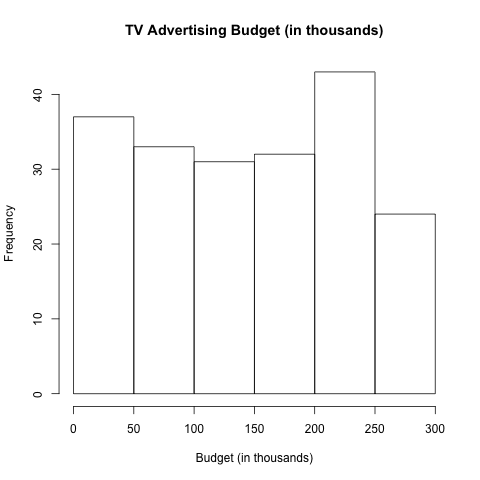
\includegraphics[width=.75\textwidth]{histogram-tv.png}
  \caption{TV Ad Budget Histogram}
\end{minipage}%
\begin{minipage}{.5\textwidth}
  \centering
  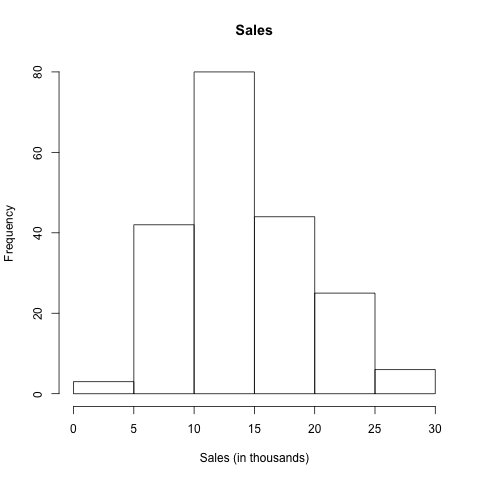
\includegraphics[width=.75\textwidth]{histogram-sales.png}
  \caption{Product Sales Histogram}
\end{minipage}
\end{figure}

As evident from Figure 1, the distribution of TV advertising budget is not normal but rather is uniform. This is good for the purposes of our invertigation of the effect of TV advertising budget on product sales because we have approximately equal representation of each TV advertising budget bucket, increasing the range of our models predictability. The distribution of product sales won't effect our model because product sales is the variable we're trying to predict. However, we see from Figure 2 that the distribution of product sales is roughly normal.

\begin{figure}[h]
\caption{Scatterplot of TV vs Sales with Regression Line}
\centering
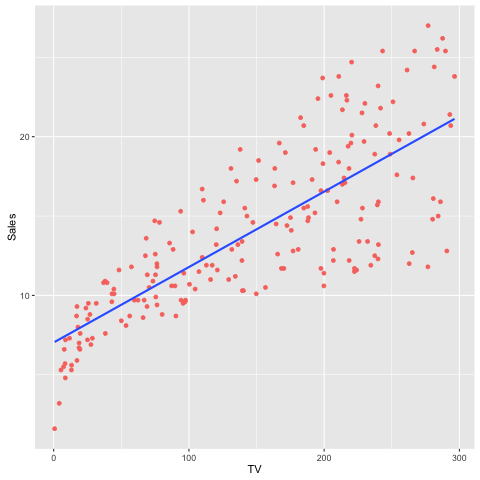
\includegraphics[width=0.35\textwidth]{scatterplot-tv-sales.png}
\end{figure}

We also must determine if the relationship between product sales and TV advertising is linear before moving forward with a simple linear regression. As evident from the scatterplot of TV advertising budget on product sales (Figure 3), the relationship is in fact linear. Thus, we can move forward with computing a simple linear regression to determine the effect of TV advertising budget on product sales.


\section{Methodology}

To assess if there is a relationship between TV advertising budget and product sales, we ran a simple linear regression of TV advertising budget on product sales--as computed in Section 3.1. We then assessed the statistical significance of the relationship between TV advertising budget and product sales using the p-value of the predictor. If the p-value of the predictor variable $X$ is less than 0.05, $X$ has a statistically significant effect on the response variable $Y$. Finally we looked at the Residual Standard Error ($RSE$), the $R^2$, and the $F-statistic$ of the model to asses the models accuracy. Because we estimate $\beta_0$ and $\beta_1$ in our model, every observation has an error term ($\epsilon$) associated with it. The $RSE$ measures the standard deviation of $\epsilon$: the average amount the predicted response will deviate from the true regression line. It's hard to interpret what a good $RSE$ is because $RSE$ is measured only in the units of $Y$. Thus, we also look at $R^2$ which measures the proportion of variance explained by the data (always a value between 0 and 1). Ideally, we'd like to see an $R^2$ that is close to 1, though this may not always be realistic depending on the question being asked. We can also assess our model's accuracy by looking at the $F-statistic$ which tests the full model (including the predictor variable $X$) against the minimalist model that assumes all values of $X$ to be zero and uses only the mean of the values in $Y$ ($\beta_0$). Associated with an $F-statistic$ is a p-value. If this p-value is less than 0.05, there is little chance that the values of the predictor $X$ are zero and thus the full model is more accurate than the minimalist model.

\section{Results}

The simple linear regression of TV advertising budget on product sales tells us that TV advertising budget has a statistically significant effect on product sales since the p-value of TV (<2e-16) is less than 0.05. This p-value can be seen in the summary statistics of the simple linear regression in Table 2. 

\begin{table}[!htbp] \centering 
  \caption{} 
  \label{} 
\begin{tabular}{@{\extracolsep{5pt}} ccccc} 
\\[-1.8ex]\hline 
\hline \\[-1.8ex] 
 & Estimate & Std. Error & t value & Pr(\textgreater \textbar t\textbar ) \\ 
\hline \\[-1.8ex] 
(Intercept) & $7.033$ & $0.458$ & $15.360$ & $0$ \\ 
TV & $0.048$ & $0.003$ & $17.668$ & $0$ \\ 
\hline \\[-1.8ex] 
\end{tabular} 
\end{table} 


From Table 2, we also see that a \$1,000 increase in TV advertising budget increases product sales. Thus, if you want to increase product sales, spending up to \$296,400 on TV advertising will do that. Note that this is only true for spending up to \$296,400 on TV advertising because this is the highest amount spent on TV advertising in the dataset used to generate the simple linear regression. If you want to determine if spending more than \$296,400 on TV advertising, another simple linear model will have to be computed that uses a data point having TV advertising budget greater than \$296,400.


\begin{table}[!htbp] \centering 
  \caption{} 
  \label{} 
\begin{tabular}{@{\extracolsep{5pt}} ccc} 
\\[-1.8ex]\hline 
\hline \\[-1.8ex] 
 & Quantity & value \\ 
\hline \\[-1.8ex] 
1 & Residual standard error & 3.259 \\ 
2 & R squared & 0.612 \\ 
3 & F-statistic & 312.145 \\ 
\hline \\[-1.8ex] 
\end{tabular} 
\end{table} 


We are also confident that the simple linear model of TV advertising budget on product sales is accurate based on the models $RSE$, $R^2$, and $F-statistic$ (shown in Table 3). We see that the $RSE$ is 3.259, meaning that the prediction of product sales based on TV advertising budget is off by 3.259*1000 units on average. The $R^2$ of the model is 0.612 meaning roughly two-thirds of the variability in product sales is explained by the model. Finally, the $F-statistic$ is 312.145 and it's associated p-value is <2.2e-16, meaning there is very little chance that the minimalist model is moe accurate than our model.

\section{Conclusions}

From this analysis, we learned that the analysis in Section 3.1 of Chapter 3. \textit{Linear Regression} in ``An Introduction to Statistical Learning'' is reproducible--since we produced its results in this paper. Additionally, by viewing the data and methodology behind the analysis in Section 3.1, we verified that the assumptions of a simple linear regression were met by the data meaning the analysis has accurate interpretation. Thus, much information can be gained by reading Section 3.1 of Chapter 3. \textit{Linear Regression} in ``An Introduction to Statistical Learning'' because the information it presents is accurate!

\end{document}
